
\section{Introduction}
    \subsection[Controle aérien a Thaiti]{Le systeme de contrôle aérien mis en place à Tahiti}
        \subsubsection{Le système TIARE}
TIARE est un système de gestion du trafic aérien pour le centre de contrôle de Tahiti, en remplacement des systèmes vieillissants de visualisation du trafic (VIVO) et de gestion de plans de vol et d’informations générales (SIGMA). La superficie de l'espace aérien géré par le centre de contrôle de Tahiti s’étend sur 12 500 000 km2. Les situations de contrôle auxquelles doivent face les contrôleurs sont multiples, il y en a en effet à traiter les spécificités du contrôle océanique, du contrôle d’approche et inter-iles. Le système TIARE est construit à partir de plusieurs « produits sur étagère » :
\begin{itemize}
\item EUROCAT-X, système en charge du traitement radar et de la gestion plans de vols.
\item ATALIS, système en charge de la préparation des vols, de la gestion des NOTAM, et de la présentation d’informations générales au contrôleur tour et approche.
\end{itemize}

Les systèmes EUROCAT-X et ATALIS sont connectés au commutateur CAGOU, raccordé aux liaisons externes (RSFTA). ATALIS reçoit également des informations météorologiques en provenance du système local d’acquisition de ces données appelé CAOBS. EUROCAT-X est raccordé au radar secondaire du mont Marau et au réseau ACARS.

        \subsubsection{La zone ACI:\label{Aci}}
Une fonction de contrôle spécifique, nommée ACI\footnote{ACI: Area Common Interest, soit une zonne d'intérets commun} ou zone ACI, a été développée dans le système EUROCAT-X pour répondre à des besoins de contrôle. Il s’agit d’une zone particulière limitrophe à la FIR\footnote{\label{FIR} la FIR est la zone dans laquelle les contrôleurs doivent assurer le contrôle des vols} de Tahiti , dons la limite se situe à 50 miles nautiques de la FIR. La zone ACI encercle la FIR. Il est à noter que cette zone n’est pas sous la responsabilité des contrôleurs aériens français, cependant, les vols pénétrant dans cette région sont visualisés par le système Eurocat-X 

Ainsi en visualisant le trafic aérien dans la zone ACI, les contrôleurs peuvent maintenir les séparations entre les aéronefs. C'est-à-dire vérifier que les vols qui sont à l’extérieur et longent la FIR de Tahiti sont séparés des vols évoluant dans cette FIR.

\section{Les objectifs et besoins du projet}
    \subsection{L'objectif initial du projet}
L’objectif principal est de pouvoir réaliser un logiciel banalisé et ergonomique permettant de
représenter l’ensemble des données de contrôle (repères, balises, secteurs...) afin de pouvoir
visualiser le trafic aérien circulant dans la FIR et la zone ACI.
Les bénéfices attendus de cet outil sont :
\begin{itemize}
\item l’amélioration de l’analyse et de la compréhension visuelle du trafic aérien de Tahiti,
\item la possibilité d’élaborer de statistiques à partir des fonctions de calcule du logiciel,
\item une aide dans le travail de définition des points d’entrée dans la zone ACI que réalise le
service de contrôle de Tahiti.
\end{itemize}

    \subsection{Le besoin}
        \subsubsection{Le besoin au début du projet}
Le besoin était initialement de pouvoir visualiser les plans de vol des avions afin de pouvoir aider les contrôleurs à déterminer l'heure d'entrée approximative de l'avion dans la zone ACI (cf. \vref{Aci})
Le logiciel devant être portable et adaptable, l'utilisation langage Python a été défini comme l'une des meilleur alternative.
Tout au long du projet de nouveau besoin se sont fait ressentir. Ceux-ci comme nous pourrons le constater dans la suite du rapport nous a amener à modifier les objectifs du projet.

        \subsubsection{Un besoin redéfinit tout au long du projet}
On a très vite constaté, ce e dès les premières représentations,  que la création d'un logiciel qui pouvait représenter les données du système TIARE dans Google Eath pourrait avoir plusieurs intérêts:
\begin{itemize}
\item Visualiser comment le Système interprète les données
\item Comparer les plan de vol déposé avec les vols réalisé
\item Visualiser les zone de contrôles
\item Évaluer la mise en place du système ADS
\end{itemize}
C'est pourquoi les besoins on été redéfinit en cours de projet.

        \subsubsection{Des besoins redéfinis}
Les nouveaux besoins définis sont donc de pouvoir disposer d'une maquette (Appellée en anglais: Poc\footnote{Proof of concept: démonstration de faisabilité}) qui serrait représentative de toutes les possibilités que pourrait apporter un logiciel de ce type.

Cette maquette doit être capable de:
\begin{itemize}
\item définir un point d'entré approximatif d'un plan de vol dans la zone ACI.
\item Visualiser les zone de contrôles
\item Visualiser tous les points caractéristique du système (Aéroport, balises …)
\item Visualiser les routes définie dans le système.
\item Visualiser les plan de vol en fonction du temps
\item Visualiser les report ADS ainsi que les points calculés par le système TIARE
\item Différencier les vols interne, sortant, entrant et en transit.
\end{itemize}

L’intérêt de cette maquette serrait de définir les spécification d'un logiciel qui pourrait être ensuite réalisé et mis en production dans des sites ou la sécurité n'est pas à négliger. Il aurait aussi l’intérêt de définir les fonctionnalités nécessaires à un utilisateur donné.

\section{La réalisation du projet}
    \subsection{La méthodologie appliqué}
Pour la réalisation de ce projet, vue les circonstance, une méthodologie existante c'est mise en place automatiquement. Celle ci est l'Extreme programming\footnote{L'Extreme Programming a été inventée par Kent Beck, Ward Cunningham et Ron Jeffries pendant leur travail sur un projet « C3 » de calcul des rémunérations chez Chrysler. Kent Beck, chef de projet en mars 1996 commença à affiner la méthodologie de développement utilisée sur le projet. La méthode est née officiellement en octobre 1999 avec le livre Extreme Programming Explained de Kent Beck. "Wikipedia"} décrite ci-après.

Dans les méthodes traditionnelles, les besoins sont définis et souvent fixés au départ du projet informatique ce qui accroît les coûts ultérieurs de modifications. Extreme programming s'attache à rendre le projet plus flexible et ouvert au changement en introduisant des valeurs de base, des principes et des pratiques.

L'Extreme Programming repose sur des cycles rapides de développement (des itérations de quelques semaines voir dans notre cas quelques jours seulement) dont les étapes sont les suivantes:
\begin{itemize}
\item une phase d'exploration détermine les scénarios clients qui seront fournis pendant cette itération,
\item la transformation des scénarios en tâches à réaliser et en tests fonctionnels,
\item lorsque tous les tests fonctionnels passent, le produit est livré.
\end{itemize}

Lorsqu'une tâche est terminée, les modifications sont immédiatement intégrées dans le produit complet. On évite ainsi la surcharge de travail liée à l'intégration de tous les éléments avant la livraison. Les tests facilitent grandement cette intégration: quand tous les tests passent, l'intégration est terminée.

Le cycle se répète tant que le client peut fournir des scénarios à livrer (cf. Fig. \vref{XP}). Généralement le cycle de la première livraison se caractérise par sa durée et le volume important de fonctionnalités embarquées. Après la première mise en production, les itérations peuvent devenir plus courtes (par exemple la séparation des plans de vol en catégories tel que: transit, interne …)
\begin{figure}
\center
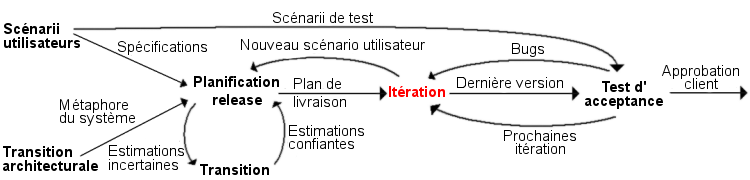
\includegraphics[width=15cm]{images/xp.png}
\caption{Cycle de l'Exreme Programing.}
\label{XP}
\end{figure}

Il est bien entendu qu'avant de passer a la pratique un apprentissage théorique a du etre réalisé comme par exemple:
\begin{itemize}
\item L'apprentissage des bonnes manières de coder en python (cf. \vref{pygood}),
\item Le fonctionnement des fichier KML (cf. %\vref{KML})
\item Ou encore les formule mathématique permettant de trouver l'intersection de deux arc de cercle en coordonnées sphérique (cf. %\vref{coord}).
\end{itemize}
    \subsection{L'apprentissage}
Avant chaque intervention sur le code une étape apprentissage a été nécessaire, dans cette partie serra décrite les partie qui m'ont le plus sollicitées.

        \subsubsection{Le langage Python}
            \paragraph{Bien coder:\label{pygood}}
Afin de pouvoir apprendre les bonne pratique de la programmation Python\cite{pybook} j'ai lu (en diagonale) un livre tres bien expliqué intitulé Programation Python, conception et Optimisation. Celui-ci m'a permit de pouvoir d'une part revoir ce qui avait été appliquer lors de mes etudes et d'autre part avoir une vue global sur le langage et ainsi pouvoir prendre du recule lors du codage.

Celui ci m'a par exemple appris le nouveau style de programmation qui part du principe que chaque nouvel objet définit est basé sur un Objet existant, et que par la même occasion tout en python était Objet (même une simple variable booléene). Ou encore la maniere de verifier si un objet etait faux, egale à 0 ou encore une chaine vide simplement en demandant si il existait (ex:~\texttt{"if x != 0:"}~devient \texttt{"if not x:"})

            \paragraph{Utiliser les expression régulière:} 
L'apprentissage de l'utilisation des expression réguliere\footnote{Une expression régulière
 est en informatique une chaîne de caractères que l’on appelle parfois un motif et qui décrit un ensemble de chaînes de caractères possibles selon une syntaxe précise.}, m'a été grandement facilité garce au site: \url{http://www.dsimb.inserm.fr/}\cite{re} et a la documentation en ligne de Python\cite{pydoc}. Il s'est avéré après apprentissage que ces expression régulière auron grandement facilité la faisabilité du projet.

            \paragraph{L'optimisation:} 
Je pourrais cité un passage du livre qui dit:
\begin{quotation}
Fourni dès le départ avec des modules de tests, Python est un langage agile. Le terme agile est originellement issu de la méthodologie de programmation agile (Beck et Al.), très proche de la programmation itérative. Cette méthodologie, qui réduit les risques liés à la conception de logiciels, introduit entre autres des principes de tests continus du code.
\raggedleft Vincent \textsc{Lozano}.
\end{quotation}

En effet il m'a été rapidement nécessaire de réalisé des test, aussi bien pour vérifier que mon code etait valide que pour vérifier que celui-ci s’exécutait normalement. Il c'est avéré a plusieurs reprise que certaine partie de mon code était très gourmande en processus %(cf : BLABLA)
. L’apprentissage des fonction de test poussé du code tel que le module hotshot décrit plus tard %(cf : BLABLA) 
m'a été rapidement nécessaire.

        \subsubsection{Le domaine de l'aviation}
Il m'a aussi été nécessaire de prendre connaissance de touts les terme, unité, convention et j'en passe utilisé dans le domaine aéronautique.

            \paragraph{Les coordonnées et unités:}
Tout d'abord est vite venu le problème de conversion de coordonnées, J'ai donc du revoir les conversions de coordonnées sphériques ainsi que les conversions de distances.
J'ai également du, comme expliquée ci dessus %(cf : BLABLABLA) 
me remémoré les manière de calculé le point d'intersection de deux arc de cercle en coordonnées sphériques.

           \paragraph{Convention:}
Plusieurs conventions on du être acquise comme celle utilisé par le système TIARE pour décrire les report ADS ou encre celle utilisée par les compagnie pour le dépôt de plan de vole.
NE PAS OUBLIER DE FAIR REF AU DOCUMLENT 4444 ...

        \subsubsection{\textsc{Google Erath}}
\textsc{Google Erath} est un logiciel, propriété de la société \textsc{Google}, permettant une visualisation de la terre en 3 dimensions avec un assemblage de photographies aériennes ou satellitaires. Ce logiciel donne la possibilité de configurer un environement, ajouter des lignes, des points ou encore des polygone en 3D en passent par des fichier de configuration au format KML\footnote{KML: Keyhole Markup Language, est un format de fichier et de grammaire XML pour la modélisation et le stockage de caractéristiques géographiques comme les points, les lignes, les images, les polygones et les modèles pour l'affichage dans \textsc{Google Erath}, dans \textsc{Google Maps} et dans d'autres applications.}.

Ce format, qui repose sur le XML\footnote{XML: Extensible Markup Language («langage extensible de balisage»), est un langage informatique de balisage générique.}, a l'avantage d’être simple à manipuler. Ça sémantique est définie sur le de google (cf. Biliographie \cite{gecode}) 

